\chapter{Introduction}

\section{État de l'art}
\blindtext[10]

\section{Les loutres}
\blindtext[6]

\begin{figure}[tb]
\begin{center}
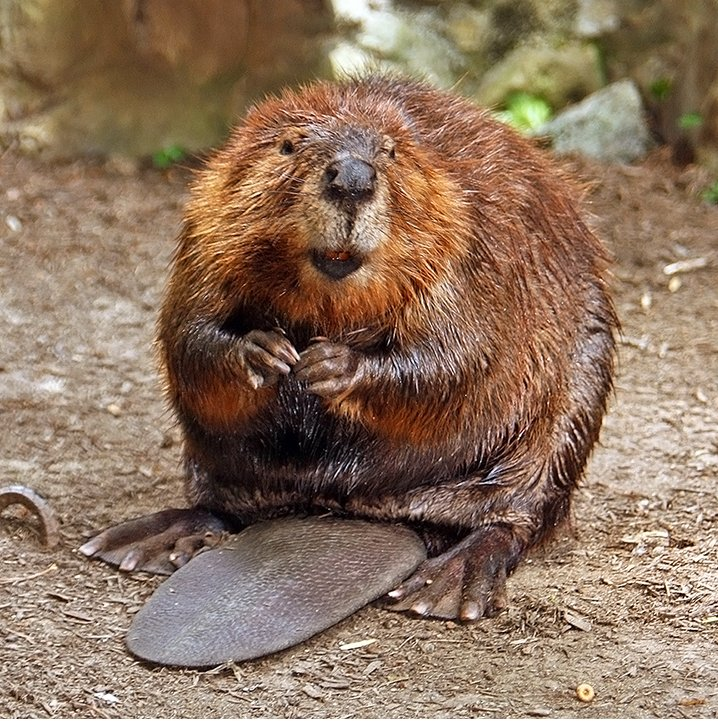
\includegraphics[width = .45 \textwidth]{introduction/figures/castor.jpg}
\end{center}
\caption{Un castor d’Amérique.}
\label{fig:castor}
\end{figure}

\begin{figure*}[tb]
\begin{center}
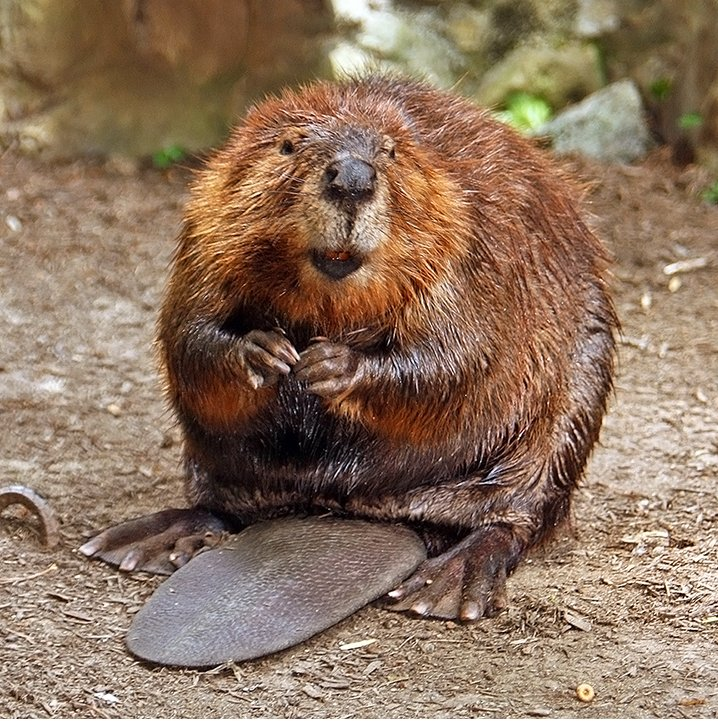
\includegraphics[width = .8\textwidth]{introduction/figures/castor.jpg}
\end{center}
\caption{Un {\huge gros} castor d’Amérique.}
\label{fig:groscastor}
\end{figure*}

\begin{figure}[h!]
\begin{center}
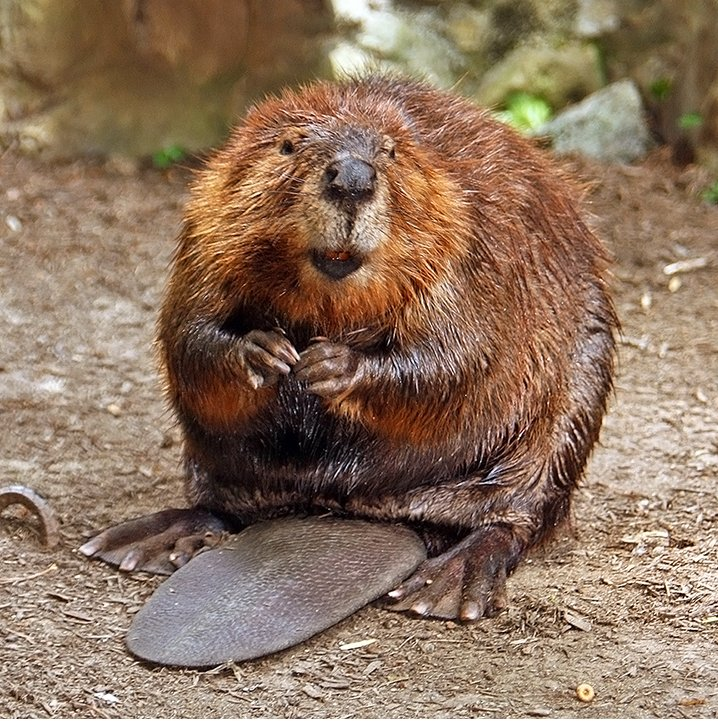
\includegraphics[angle = 45., width = .3\textwidth]{introduction/figures/castor.jpg}
\label{fig:castornonflotant}
\end{center}
\caption{Un castor qui ne flotte pas d’Amérique.}
\label{fig:groscastor}
\end{figure}

\blindtext[10]